\documentclass[]{article}
\usepackage{lmodern}
\usepackage{amssymb,amsmath}
\usepackage{ifxetex,ifluatex}
\usepackage{fixltx2e} % provides \textsubscript
\ifnum 0\ifxetex 1\fi\ifluatex 1\fi=0 % if pdftex
  \usepackage[T1]{fontenc}
  \usepackage[utf8]{inputenc}
\else % if luatex or xelatex
  \ifxetex
    \usepackage{mathspec}
  \else
    \usepackage{fontspec}
  \fi
  \defaultfontfeatures{Ligatures=TeX,Scale=MatchLowercase}
    \setsansfont[]{Times New Roman}
\fi
% use upquote if available, for straight quotes in verbatim environments
\IfFileExists{upquote.sty}{\usepackage{upquote}}{}
% use microtype if available
\IfFileExists{microtype.sty}{%
\usepackage{microtype}
\UseMicrotypeSet[protrusion]{basicmath} % disable protrusion for tt fonts
}{}
\usepackage[margin=1in]{geometry}
\usepackage{hyperref}
\hypersetup{unicode=true,
            pdftitle={STA303 Assignment2},
            pdfauthor={Guanchen Zhang},
            pdfborder={0 0 0},
            breaklinks=true}
\urlstyle{same}  % don't use monospace font for urls
\usepackage{graphicx,grffile}
\makeatletter
\def\maxwidth{\ifdim\Gin@nat@width>\linewidth\linewidth\else\Gin@nat@width\fi}
\def\maxheight{\ifdim\Gin@nat@height>\textheight\textheight\else\Gin@nat@height\fi}
\makeatother
% Scale images if necessary, so that they will not overflow the page
% margins by default, and it is still possible to overwrite the defaults
% using explicit options in \includegraphics[width, height, ...]{}
\setkeys{Gin}{width=\maxwidth,height=\maxheight,keepaspectratio}
\IfFileExists{parskip.sty}{%
\usepackage{parskip}
}{% else
\setlength{\parindent}{0pt}
\setlength{\parskip}{6pt plus 2pt minus 1pt}
}
\setlength{\emergencystretch}{3em}  % prevent overfull lines
\providecommand{\tightlist}{%
  \setlength{\itemsep}{0pt}\setlength{\parskip}{0pt}}
\setcounter{secnumdepth}{0}
% Redefines (sub)paragraphs to behave more like sections
\ifx\paragraph\undefined\else
\let\oldparagraph\paragraph
\renewcommand{\paragraph}[1]{\oldparagraph{#1}\mbox{}}
\fi
\ifx\subparagraph\undefined\else
\let\oldsubparagraph\subparagraph
\renewcommand{\subparagraph}[1]{\oldsubparagraph{#1}\mbox{}}
\fi

%%% Use protect on footnotes to avoid problems with footnotes in titles
\let\rmarkdownfootnote\footnote%
\def\footnote{\protect\rmarkdownfootnote}

%%% Change title format to be more compact
\usepackage{titling}

% Create subtitle command for use in maketitle
\newcommand{\subtitle}[1]{
  \posttitle{
    \begin{center}\large#1\end{center}
    }
}

\setlength{\droptitle}{-2em}

  \title{STA303 Assignment2}
    \pretitle{\vspace{\droptitle}\centering\huge}
  \posttitle{\par}
    \author{Guanchen Zhang}
    \preauthor{\centering\large\emph}
  \postauthor{\par}
      \predate{\centering\large\emph}
  \postdate{\par}
    \date{August 4, 2018}

\usepackage{amsmath}
\usepackage{commath}
\usepackage{geometry}
\geometry{top=1in}

\begin{document}
\maketitle

\fontsize{12}{12}

\subsection{Dataset 1}\label{dataset-1}

To predict whether prostate cancer has spread to neighbouring lymph
node, we recorded and studied five binary explanatory variables of 53
patients with prostate cancer. The five binary explanatory variables
include: age (0 = less than 60, 1 = 60 or more); stage (0=less serious
tumour, 1 = more serious); grade (0=less serious patholohy of
tumour,1=more serious); xray (0=less serious, 1=more serious); acid
(0=less than 0.6 of serum acid phosphatase, 1=0.6 or more).

It is not possible to make a causal conclusion about the relationship of
each predicor with nodal involvement based on these data because the
purpose for regression is to study the correlation relationships,
however, correlation does not necessary mean causation, which tries to
estimate the effect of intervention.

We want to do a predictive anlysis on nodal involvment, therefore,
regression analysis should be used. Since the dependent variable (r in
this context) is binary, logistic regression is most appropriate to use.
The binary logistic regression model assumes 1) the dependent variable
should be dichotomous 2) the observations to be independent of each
other 3) little or not multicollinearity among the independent variables
4)There is a linear relationship between the logit of the outcome and
each predictor variables 5)\(Var(y_i) = n_ip_i(1-p_i)\). The assumption
1) and 2) is satisfied because each data entry means an individual.
Based on the correlation matrix (table 1.2), there is little
multicollinearity among the independent variables. The linearity
assumption holds based on Figure 1.1, the smoothed scatter plots show
that variables are linearly associated with the outcome in logit scale,
but since the sample size is small, the result is not informative.

By performing a stepwise variable selection, we can get a simpler model
(nodal\_glm2) that is better than a model including all predictors
(nodal\_glm). In detail, we build regression model from a set of
candidate predictor variables by entering predictors in a stepwise
manner into a null model where AIC criterion is used for evaluating
subsets of variables. Comparing the AIC of nodal\_glm model (59.611) to
AIC of simpler model (57.18), the simpler nodal\_glm2 indeed is better.
The reason to compare AIC instead of deviance is that larger model
always implies smaller deviance but AIC compensate for that. Hence, we
are suggested that only predictors of stage, xray and acid have a
apparent relationship with nodal involvment. Then we performed the
likelihood ratio test, the simpler mode fits as well as the saturated
model and better than null model. Also, the null model doesn't fit the
data as well as the saturated model. However, we should not rely on this
goodness-of-fit measurement because deviance depends on beta\_hat rather
than contrasting the data with fitted model. Another reason is that if
the data are modelled into binomial format, the degrees of freedom of
fitted model would change.

To conclude, though the spread of cancer to neighbouring lymph nodes for
patients with prostate cancer seems to have a relationship with
seriousness of tumour(stage),xray and level of serum acid
phosphatase(acid), we still cannot make a conclusive treatment strategy
because of lack of data and low reliability on goodness-of-fit
measurement of binary data.

\subsection{Appendix 1}\label{appendix-1}

\paragraph{Table 1.1 Glimpse data}\label{table-1.1-glimpse-data}

\begin{verbatim}
## Observations: 53
## Variables: 7
## $ m     <dbl> 1, 1, 1, 1, 1, 1, 1, 1, 1, 1, 1, 1, 1, 1, 1, 1, 1, 1, 1,...
## $ r     <dbl> 1, 1, 1, 1, 1, 0, 1, 0, 0, 0, 0, 0, 0, 0, 0, 0, 1, 1, 0,...
## $ aged  <fct> 0, 0, 0, 0, 0, 0, 0, 0, 0, 0, 0, 0, 1, 1, 1, 1, 1, 1, 1,...
## $ stage <fct> 1, 1, 1, 1, 1, 1, 0, 0, 0, 0, 0, 0, 1, 1, 1, 1, 1, 1, 1,...
## $ grade <fct> 1, 1, 1, 1, 1, 1, 0, 0, 0, 0, 0, 0, 1, 1, 1, 1, 0, 0, 0,...
## $ xray  <fct> 1, 1, 1, 1, 1, 1, 0, 0, 0, 0, 0, 0, 0, 0, 0, 0, 0, 0, 0,...
## $ acid  <fct> 1, 1, 1, 1, 1, 1, 1, 1, 1, 1, 1, 1, 0, 0, 0, 0, 1, 1, 1,...
\end{verbatim}

\paragraph{Table 1.2 Correlation matrix of
predictors}\label{table-1.2-correlation-matrix-of-predictors}

\begin{verbatim}
##        aged stage grade  xray  acid
## aged   1.00  0.06 -0.19 -0.10 -0.20
## stage  0.06  1.00  0.41  0.15  0.13
## grade -0.19  0.41  1.00  0.22  0.01
## xray  -0.10  0.15  0.22  1.00  0.16
## acid  -0.20  0.13  0.01  0.16  1.00
\end{verbatim}

\begin{verbatim}
## 
## Call:
## glm(formula = r ~ aged + stage + grade + xray + acid, family = binomial, 
##     data = nodal_tbl)
## 
## Deviance Residuals: 
##     Min       1Q   Median       3Q      Max  
## -2.3317  -0.6653  -0.2999   0.6386   2.1502  
## 
## Coefficients:
##             Estimate Std. Error z value Pr(>|z|)   
## (Intercept)  -8.5173     2.8259  -3.014  0.00258 **
## aged         -0.2917     0.7540  -0.387  0.69881   
## stage         1.3729     0.7838   1.752  0.07986 . 
## grade         0.8720     0.8156   1.069  0.28500   
## xray          1.8008     0.8104   2.222  0.02628 * 
## acid          1.6839     0.7915   2.128  0.03337 * 
## ---
## Signif. codes:  0 '***' 0.001 '**' 0.01 '*' 0.05 '.' 0.1 ' ' 1
## 
## (Dispersion parameter for binomial family taken to be 1)
## 
##     Null deviance: 70.252  on 52  degrees of freedom
## Residual deviance: 47.611  on 47  degrees of freedom
## AIC: 59.611
## 
## Number of Fisher Scoring iterations: 5
\end{verbatim}

\begin{verbatim}
## Start:  AIC=59.61
## r ~ aged + stage + grade + xray + acid
## 
##         Df Deviance    AIC
## - aged   1   47.760 57.760
## - grade  1   48.760 58.760
## <none>       47.611 59.611
## - stage  1   50.808 60.808
## - acid   1   52.660 62.660
## - xray   1   52.922 62.922
## 
## Step:  AIC=57.76
## r ~ stage + grade + xray + acid
## 
##         Df Deviance    AIC
## - grade  1   49.180 57.180
## <none>       47.760 57.760
## - stage  1   50.817 58.817
## - xray   1   53.162 61.162
## - acid   1   53.526 61.526
## 
## Step:  AIC=57.18
## r ~ stage + xray + acid
## 
##         Df Deviance    AIC
## <none>       49.180 57.180
## - acid   1   54.463 60.463
## - stage  1   54.788 60.788
## - xray   1   55.915 61.915
\end{verbatim}

\begin{verbatim}
## 
## Call:
## glm(formula = r ~ stage + xray + acid, family = binomial, data = nodal_tbl)
## 
## Deviance Residuals: 
##     Min       1Q   Median       3Q      Max  
## -2.1231  -0.6620  -0.3039   0.4710   2.4892  
## 
## Coefficients:
##             Estimate Std. Error z value Pr(>|z|)    
## (Intercept)  -8.2465     2.2224  -3.711 0.000207 ***
## stage         1.6453     0.7297   2.255 0.024139 *  
## xray          1.9116     0.7771   2.460 0.013900 *  
## acid          1.6378     0.7539   2.172 0.029834 *  
## ---
## Signif. codes:  0 '***' 0.001 '**' 0.01 '*' 0.05 '.' 0.1 ' ' 1
## 
## (Dispersion parameter for binomial family taken to be 1)
## 
##     Null deviance: 70.252  on 52  degrees of freedom
## Residual deviance: 49.180  on 49  degrees of freedom
## AIC: 57.18
## 
## Number of Fisher Scoring iterations: 5
\end{verbatim}

\begin{verbatim}
## [1] 0.0001017218
\end{verbatim}

\begin{verbatim}
## [1] 0.4658993
\end{verbatim}

\begin{verbatim}
## [1] 0.0466085
\end{verbatim}

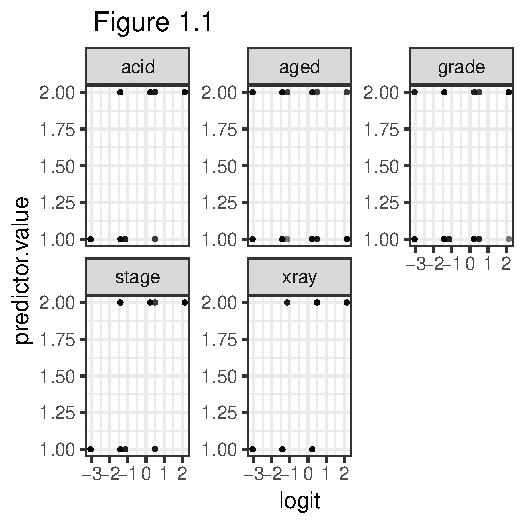
\includegraphics{a2_files/figure-latex/unnamed-chunk-6-1.pdf}

\subsection{Dataset 2}\label{dataset-2}

To study how age, smoking and survival related to each other, these 3
factors of 1314 women in Whickham were recorded in 1972-1974 and twenty
years later a follow-up survey was conducted to determine the mortality
of the origin participants.

In this context, because the relationship between the variables is more
symmetric and there is no implicitly assumption on association between
smoer and age, poisson regression model is preferred to investigate how
3 factors interact. If we want one factor being identified as the
response, we would prefer binomial model but it is not our case.
Therefore, we need to transform the original data frame to fit a poisson
model (table2.4). Firstly, we consider if all 3 variables are
independent, say, mutual independence, corresponding to the main
effects-only model smoke\_glm1. Then considering the joint independence,
though there are many possible case, we prefer to suppose smoking and
death are dependent but jointly independent of age which makes most
sense. This represents a small improvement over mutual independence
since XXX, but the degree of freedom of deviance is still high. Finally,
we consider the conditional independence which suppose smoking is
independent of life status given age. The deviance is slightly larger
than degree of freedon and smaller than the deviance of previous 2
models, indicating a better fit.

From Table2.3, 76\% smokers have survived for 20 years while only 69\%
nonsmokers have survived, which intuitively indicating smoking have a
beneficial effect. But once we consider the relationship within age
group, the advantage to nonsmoker over smoker is obvious. From table2.1
and 2.2, within the same age group, there are always more smokers died
than nonsmokers. There is a difference between the case when we
marginalize the age and the case when we control for age, which might
result from the fact that smokers are more concentrated in the younger
age group and old people were more likely to pass away after 20 years no
matter whether they smoke or not. Therefore, it is dangerous to
ignore/marginalize over variables without first examining the full
dependence structure. For example in this case, marginalizing the age
group veils the condition for dependence structure, ending up with the
opposite experiment result.

To conclude, in 20 year long period, smoking is independent of life
status given age and within each age group, smoking has a harmful effect
on life status compared to nonsmoking.

\subsection{Appendix 2}\label{appendix-2}

\paragraph{Table 2.1}\label{table-2.1}

\begin{verbatim}
## , ,  = dead
## 
##       age
## smoker 18-24 25-34 35-44 45-54 55-64 65-74 75+
##      0     1     5     7    12    40   101  64
##      1     2     3    14    27    51    29  13
## 
## , ,  = alive
## 
##       age
## smoker 18-24 25-34 35-44 45-54 55-64 65-74 75+
##      0    61   152   114    66    81    28   0
##      1    53   121    95   103    64     7   0
\end{verbatim}

\paragraph{Table 2.2}\label{table-2.2}

\begin{verbatim}
## , ,  = dead
## 
##       age
## smoker 18-24 25-34 35-44 45-54 55-64 65-74  75+
##      0  0.01  0.02  0.03  0.06  0.17  0.61 0.83
##      1  0.02  0.01  0.06  0.13  0.22  0.18 0.17
## 
## , ,  = alive
## 
##       age
## smoker 18-24 25-34 35-44 45-54 55-64 65-74  75+
##      0  0.52  0.54  0.50  0.32  0.34  0.17 0.00
##      1  0.45  0.43  0.41  0.50  0.27  0.04 0.00
\end{verbatim}

\paragraph{Table 2.3}\label{table-2.3}

\begin{verbatim}
##       
## smoker dead alive
##      0 0.31  0.69
##      1 0.24  0.76
\end{verbatim}

\paragraph{Table 2.4 Transformed data
frame}\label{table-2.4-transformed-data-frame}

\begin{verbatim}
## Observations: 28
## Variables: 4
## $ y      <dbl> 2, 53, 1, 61, 3, 121, 5, 152, 14, 95, 7, 114, 27, 103, ...
## $ age    <fct> 18-24, 18-24, 18-24, 18-24, 25-34, 25-34, 25-34, 25-34,...
## $ smoker <dbl> 1, 1, 0, 0, 1, 1, 0, 0, 1, 1, 0, 0, 1, 1, 0, 0, 1, 1, 0...
## $ dead   <dbl> 1, 0, 1, 0, 1, 0, 1, 0, 1, 0, 1, 0, 1, 0, 1, 0, 1, 0, 1...
\end{verbatim}

\begin{verbatim}
## 
## Call:
## glm(formula = y ~ smoker + age + dead, family = poisson, data = smoking_tbl2)
## 
## Deviance Residuals: 
##     Min       1Q   Median       3Q      Max  
## -7.9306  -5.3175  -0.5514   2.4229  11.1895  
## 
## Coefficients:
##             Estimate Std. Error z value Pr(>|z|)    
## (Intercept)  3.84748    0.09721  39.580  < 2e-16 ***
## smoker      -0.22931    0.05554  -4.129 3.64e-05 ***
## age25-34     0.87618    0.11003   7.963 1.67e-15 ***
## age35-44     0.67591    0.11356   5.952 2.65e-09 ***
## age45-54     0.57536    0.11556   4.979 6.40e-07 ***
## age55-64     0.70166    0.11307   6.206 5.45e-10 ***
## age65-74     0.34377    0.12086   2.844  0.00445 ** 
## age75+      -0.41837    0.14674  -2.851  0.00436 ** 
## dead        -0.94039    0.06139 -15.319  < 2e-16 ***
## ---
## Signif. codes:  0 '***' 0.001 '**' 0.01 '*' 0.05 '.' 0.1 ' ' 1
## 
## (Dispersion parameter for poisson family taken to be 1)
## 
##     Null deviance: 1193.9  on 27  degrees of freedom
## Residual deviance:  735.0  on 19  degrees of freedom
## AIC: 887.2
## 
## Number of Fisher Scoring iterations: 6
\end{verbatim}

\begin{verbatim}
## 
## Call:
## glm(formula = y ~ smoker * dead + age, family = poisson, data = smoking_tbl2)
## 
## Deviance Residuals: 
##     Min       1Q   Median       3Q      Max  
## -8.2606  -5.1564  -0.5933   2.5373  10.4236  
## 
## Coefficients:
##             Estimate Std. Error z value Pr(>|z|)    
## (Intercept)  3.79994    0.09888  38.428  < 2e-16 ***
## smoker      -0.12503    0.06519  -1.918  0.05511 .  
## dead        -0.78052    0.07962  -9.803  < 2e-16 ***
## age25-34     0.87618    0.11003   7.963 1.67e-15 ***
## age35-44     0.67591    0.11356   5.952 2.65e-09 ***
## age45-54     0.57536    0.11556   4.979 6.40e-07 ***
## age55-64     0.70166    0.11307   6.206 5.45e-10 ***
## age65-74     0.34377    0.12086   2.844  0.00445 ** 
## age75+      -0.41837    0.14674  -2.851  0.00436 ** 
## smoker:dead -0.37858    0.12566  -3.013  0.00259 ** 
## ---
## Signif. codes:  0 '***' 0.001 '**' 0.01 '*' 0.05 '.' 0.1 ' ' 1
## 
## (Dispersion parameter for poisson family taken to be 1)
## 
##     Null deviance: 1193.9  on 27  degrees of freedom
## Residual deviance:  725.8  on 18  degrees of freedom
## AIC: 880
## 
## Number of Fisher Scoring iterations: 6
\end{verbatim}

\begin{verbatim}
## 
## Call:
## glm(formula = y ~ smoker * age + dead * age, family = poisson, 
##     data = smoking_tbl2)
## 
## Deviance Residuals: 
##      Min        1Q    Median        3Q       Max  
## -1.30657  -0.26480  -0.00003   0.26643   1.20822  
## 
## Coefficients:
##                   Estimate Std. Error z value Pr(>|z|)    
## (Intercept)        4.10116    0.12788  32.070  < 2e-16 ***
## smoker            -0.11980    0.18523  -0.647 0.517785    
## age25-34           0.92620    0.15109   6.130 8.78e-10 ***
## age35-44           0.59889    0.15829   3.784 0.000155 ***
## age45-54           0.04791    0.17402   0.275 0.783077    
## age55-64           0.20753    0.16516   1.257 0.208911    
## age65-74          -0.79194    0.21591  -3.668 0.000245 ***
## age75+           -22.60919 5776.51885  -0.004 0.996877    
## dead              -3.63759    0.58490  -6.219 5.00e-10 ***
## smoker:age25-34   -0.11616    0.22078  -0.526 0.598789    
## smoker:age35-44    0.01536    0.22749   0.068 0.946172    
## smoker:age45-54    0.63063    0.23414   2.693 0.007074 ** 
## smoker:age55-64    0.06894    0.22643   0.304 0.760765    
## smoker:age65-74   -1.15649    0.26427  -4.376 1.21e-05 ***
## smoker:age75+     -1.47413    0.35617  -4.139 3.49e-05 ***
## age25-34:dead      0.10756    0.68613   0.157 0.875435    
## age35-44:dead      1.33977    0.62810   2.133 0.032920 *  
## age45-54:dead      2.17125    0.61128   3.552 0.000382 ***
## age55-64:dead      3.17171    0.59999   5.286 1.25e-07 ***
## age65-74:dead      4.94977    0.61512   8.047 8.49e-16 ***
## age75+:dead       26.30450 5776.51888   0.005 0.996367    
## ---
## Signif. codes:  0 '***' 0.001 '**' 0.01 '*' 0.05 '.' 0.1 ' ' 1
## 
## (Dispersion parameter for poisson family taken to be 1)
## 
##     Null deviance: 1193.9378  on 27  degrees of freedom
## Residual deviance:    8.3269  on  7  degrees of freedom
## AIC: 184.52
## 
## Number of Fisher Scoring iterations: 17
\end{verbatim}

\paragraph{Table 2.5 ANOVA table}\label{table-2.5-anova-table}

\begin{verbatim}
## Analysis of Deviance Table
## 
## Model 1: y ~ smoker + age + dead
## Model 2: y ~ smoker * dead + age
## Model 3: y ~ smoker * age + dead * age
##   Resid. Df Resid. Dev Df Deviance
## 1        19     735.00            
## 2        18     725.80  1     9.20
## 3         7       8.33 11   717.48
\end{verbatim}


\end{document}
